\documentclass[english]{tktltiki}
\usepackage[pdftex]{graphicx}
\usepackage{subfigure}
\usepackage{booktabs}
\usepackage{url}
\usepackage{amsthm,amssymb}
 \usepackage{amsmath}
\begin{document}
\onehalfspacing

\title{Observation of an office of an IT firm}
\author{P�ter Ivanics}
\date{\today}

\maketitle

\numberofpagesinformation{\numberofpages\ pages + \numberofappendixpages\ appendices}

\section{Introduction}
This short report summarizes the findings of the "Observation" assignment given on the Designing Interactive Systems course. The goal of the observation is to learn about and discover a daily experience of employees working at a software company. By software company we mean businesses, whose main purpose and aim is software development, the monetizing and selling of their solution and/or software product(s).

The main aim of the observation is to discover is the regular habits, values and challenges of the stakeholders presented on Figure \ref{stakeholder_map} in such environment. These may include internal practices at the firm, tangible or intangible means, software or hardware components, relationships or habits of individuals. 

Typically different companies have slightly different company culture. Nevertheless, the challenges, problems and some tasks faced by individual companies share similarities. For example, overcoming the challenges created by in intercultural environment, employee well-being and satisfaction, leadership, short and long term planning, time-scheduling or work-free time balance of employees are widely faced challenges along different fields. The motivation behind selecting such environment is the possibility to generalize the findings widely and project them onto a similar, but essentially different environment. Nowadays there is a high number of companies operating in software-related areas.

For convenience, the current workplace of the researcher is selected as a case company. Please note that as the sample is limited to a single company and observation and therefore the results of this report are not sufficient to generalize them onto a wide scope. To do so, further observations and other type of data collection methods, such as interviews, in various setting should be conducted and analyzed.  

\section{Stakeholder map}
The stakeholder map of the analyzed office environment is listed below (Figure \ref{stakeholder_map}). The main stakeholders to focus on are employees, employers, customers and cleaners who visit the office on a regular basis. Despite the fact that other stakeholders are displayed on the map, they are excluded from the analysis due to its reduced scope. 

	\begin{figure}[h] 
		\begin{center}
			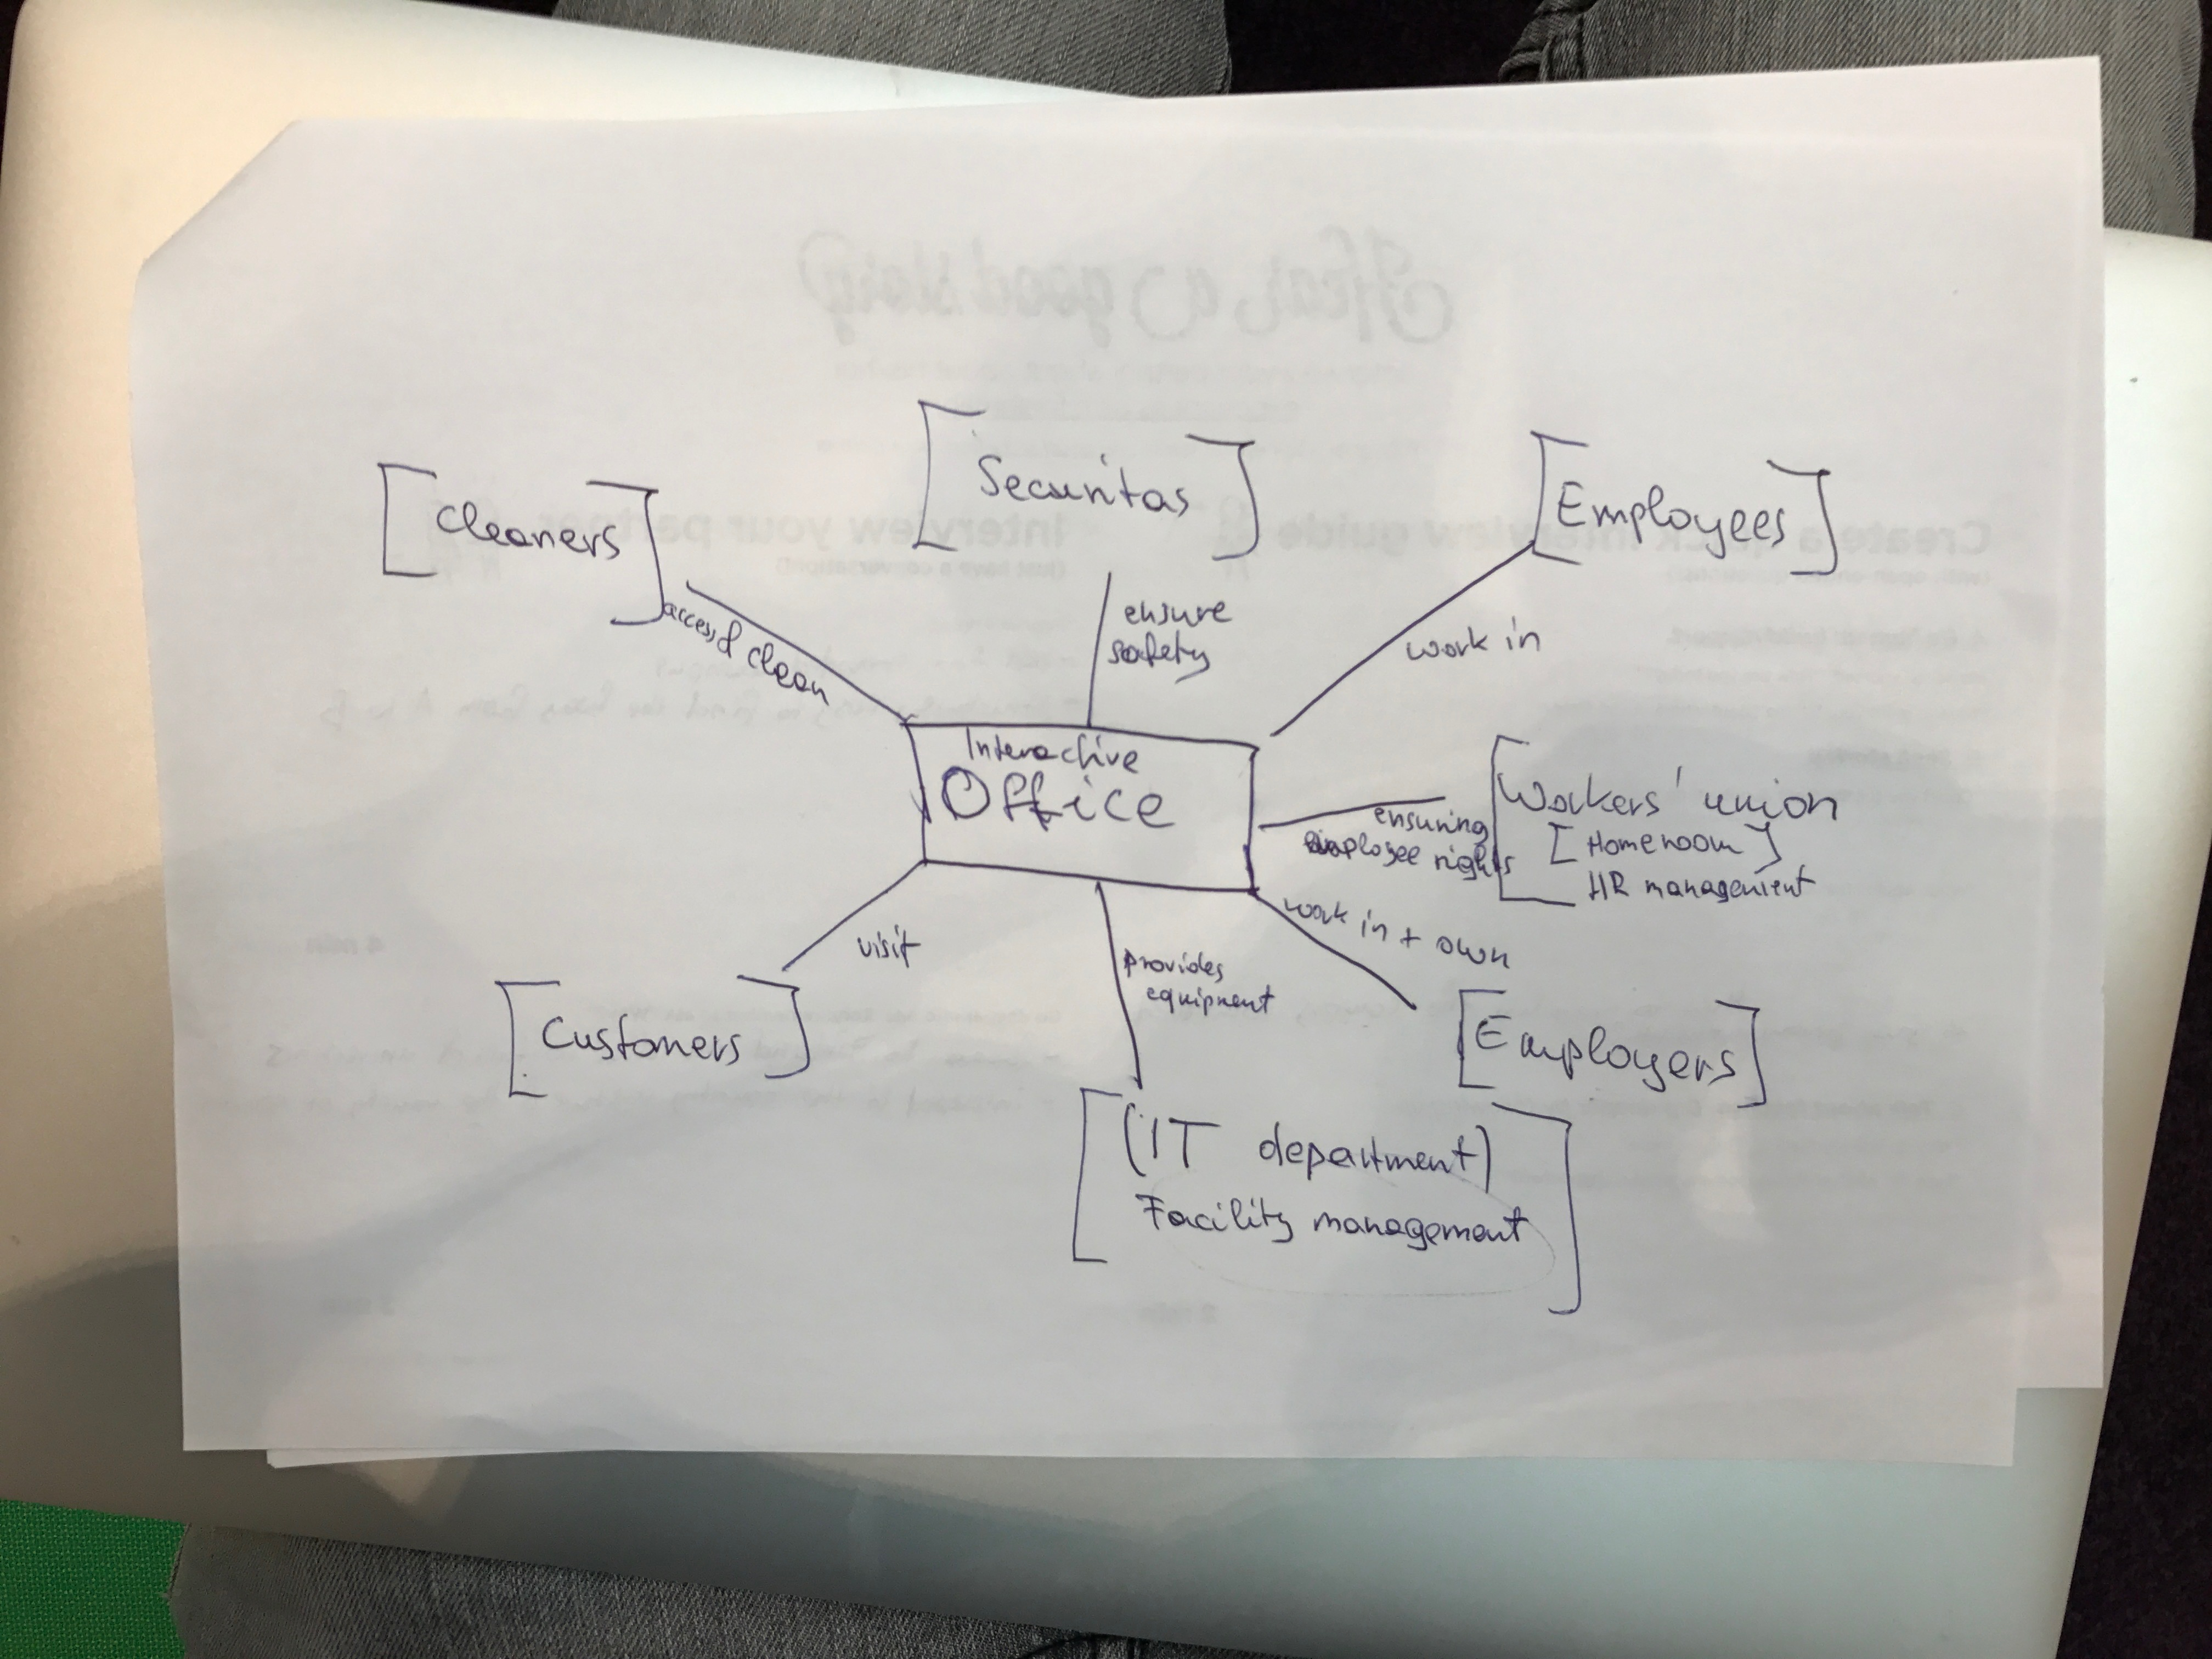
\includegraphics[width=0.9\textwidth]{images/stakeholdermap.jpg}
			\caption{The stakeholder map in an office environment.}
			\label{stakeholder_map}
		\end{center}
	\end{figure}
	
To give more understanding to the context, let us take a look at the the relationships among these stakeholders. Essentially, the above listed stakeholders visit their working environment on a regular basis to perform their job. Depending on the situation and role filled in by individuals at the firm, the regularity of visiting the office environment may differ. Nevertheless, the purpose remains the same and the "effectiveness" of the work is clearly a key aspect for all stakeholders. If one visits their work environment, their aim is to get their job done effectively. 

Effectiveness of work may depend on multiple dimensions such as how creative the work environment is, which practices employees use to cooperate, how well those practices fit their team spirit, does the environment facilitate creativity and last but not least, what is the mental state and level of well being of the involved parties. 

In this respect, there is a clear relationship between employers (supervisors) and employees which requires the establishment of an environment, that can get the best possible outcome of the team working in the office. This involves role delegation, company culture, strategy and employee satisfaction. On top of that, employers typically have the role to motivate their employers to enhance their commitment and motivation towards work. Similarly, employees may aim work an intellectually stimulating workplace by challenging themselves with professionally demanding tasks and by learning from respective colleagues. 

At the same time, employers aim to maximize business value and revenue. For this reason, it is essential to have a highly committed and motivated team behind the company strategy. Every now and then, the customers of the firm visit the office on-site and seek the trust and confidence in their business partner. Companies having such workforce unconsciously give a good impression towards the customer as the trust is established by seeing individuals' commitment and joy at their work. 

Last, but not least, cleaners play a role to maintain the hygiene of the working environment. Their aim and goals towards the office environment is different and typically do not interact too much with the employees nor the management of the company who owns the facilities. However, they visit with very similar task-list and perform similar actions on a regular (in some cases even daily) basis in multiple, similar offices. Despite the fact that there is not too many relationship between them and other stakeholders, they would benefit from solutions supporting their repetitive tasks and assist them to perform those quicker. 

\section{Observation}


\section{Conclusions}

\lastpage

\appendices

\pagestyle{empty}
\end{document}